\section*{Opgave 3}\addcontentsline{toc}{section}{Opgave 3}\refstepcounter{section}
Det �nskes at finde volumen indesluttet af cylinderen
\begin{equation*}
	x^2+y^2=4
\end{equation*}
og afgr�nset af 
\begin{align*}
	z=x+y+4\\
	z=x-y\\
	z \geq 0
\end{align*}

\begin{figure}[htb]
	\begin{center}
	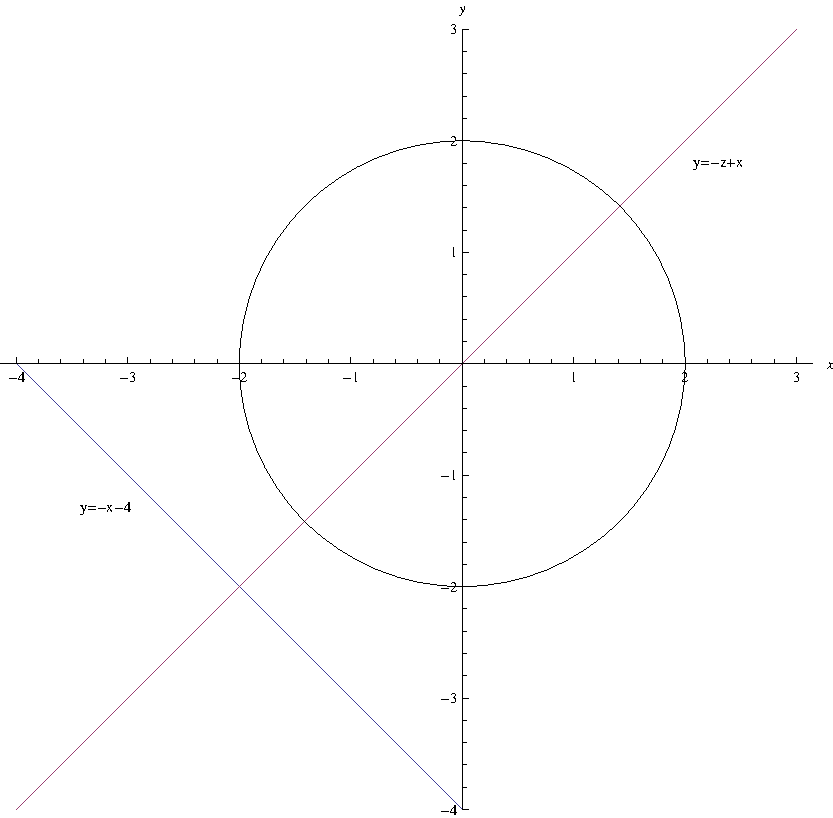
\includegraphics[width=0.7\textwidth]{opg3_z0} %trim=l b r t
	\caption{Problem afbilledet i $(x,y)$-planet hvor $z=0$}
	\label{fig:opg3_z0}
	\end{center}
\end{figure}

Cylinderen er symmetrisk om $z$-aksen (har centrum i $(0,0)$ i $(x,y)$-planet) og har radius $2$. For at f� en ide om, hvordan gr�nserne ser ud, ser vi p� $(x,y)$-planet i det $z=0$ (figur \ref{fig:opg3_z0})

P� figur \ref{fig:opg3_z0} ses det, at $z=x+y+4$ ikke ''sk�rer'' noget af cylinderen s� l�nge $z \geq 0$. Dog g�r $z=x-y$ lige igennem cylinderens midte n�r $z=0$, men fordi $z=x-y$ stiger eller falder lige meget p� begge sider af $z=0$ kan vi faktisk helt ignorere den afgr�nsning og bare bruge $z=0$. Det er ingen grund til f�rst at skulle finde den volume for s� at ''tr�kke den fra'' bagefter. Figur \ref{fig:opg3_x0} viser dette: Det skraverede omr�de er hvor $z=x-y$ er forskellig fra $z=0$ indenfor cylinderens sider.

\begin{figure}[htb]
	\begin{center}
	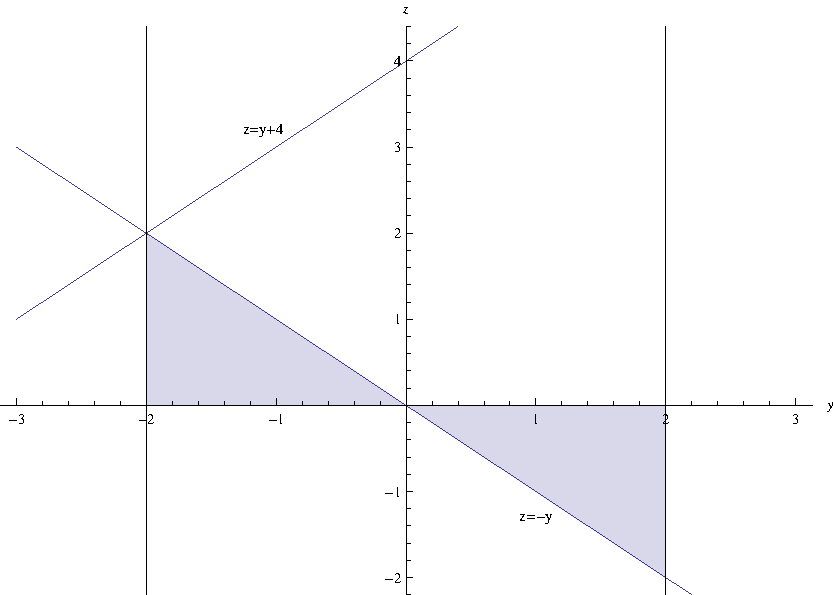
\includegraphics[width=0.84\textwidth]{opg3_x0} %trim=l b r t
	\caption{Problem afbilledet i $(z,y)$-planet hvor $x=0$. De lodrette streger er cylinderens sider.}
	\label{fig:opg3_x0}
	\end{center}
\end{figure}

Nu kan integralet s� opstilles. For at lette integrationen benyttes cylindriske koordinater. F�rst findes arealet af $r \, dz$, fra $z=0$ til vi rammer $z=x+y+4$. Radius skal summeres fra $0$ til $2$ og $\theta$ er en fuld cirkel fra $0$ til $2\pi$.
\begin{align*}
	\int_0^{2 \pi } \int_0^2 \int_0^{r \cos\theta +r \sin\theta +4} r \, dz \, dr \, d\theta 
\end{align*}

S�ledes kan vi evaluere integralet
\begin{align*}
	& \int_0^{2 \pi } \int_0^2 \int_0^{r \cos\theta +r \sin\theta +4} r \, dz \, dr \, d\theta \\
	&= \int_0^{2 \pi } \int_0^2 \left( r^2 \cos\theta + r^2 \sin\theta +4r \right) \, dr \, d\theta \\
	&= \int_0^{2 \pi } \left( \bigg[ \frac{1}{3}r^3 \cos\theta + \frac{1}{3}r^3 \sin\theta +2r^2 \bigg]_{0}^{2} \right) \, d\theta \\
	&= \int_0^{2 \pi } \left( \frac{8}{3} \cos\theta + \frac{8}{3} \sin\theta +8 \right) \, d\theta \\
	&= \bigg[ \frac{8}{3} \sin\theta - \frac{8}{3} \cos\theta +8\theta \bigg]_{0}^{2\pi} \\
	&= \left( -\frac{8}{3} + 16 \pi \right) - \left( -\frac{8}{3} \right) \\
	&= 16 \pi
\end{align*}